\section{Overview}
  \paragraph\
    In this chapter I describe about \emph{ntop}, Cassandra and implementation of Cassandra plugin for \emph{ntop}.
    I also specify design and implementation of Cassandra client for C that developed using C-python API. I have done few 
    testing of my solution that I describe in results section. 
    
  \section{\emph{ntop}}
  \emph{ntop} is open-source traffic measurement application written in C. \emph{ntop} design follow UNIX philosophy:
  applications can be divided into small independent pieces that co-operate to achieve a common goal.
  \emph{ntop} has following module
    \begin{enumerate}
     \item Packet Sniffer - Capture packet using \emph{libpcap} library and also from UNIX sockets.
     \item Packet Analyzer - Analysis packet captured by Packet Sniffer.
     \item Traffic Rules - \emph{ntop} allows traffic rules for capturing packets to filter out unnecessary packets.
     \item Report Engine - Report Engine display analyzed output in an interactive web-based user interface. 
     \item Plugins - Using plugins anyone can extend \emph{ntop} to support extra features.
    \end{enumerate}
    
     \subsection{Packet Sniffer}
      \paragraph\
	Packet Sniffer captures packet using \emph{libpcap} library and store them into internal buffer, that helps to reduce packet drops
	in a busty traffic environment. \emph{libpcap} is supported by all major Operating Systems, that allows \emph{ntop} to be 
	portable to windows and UNIX variants.
        \begin{figure}[htb]
          \centering
          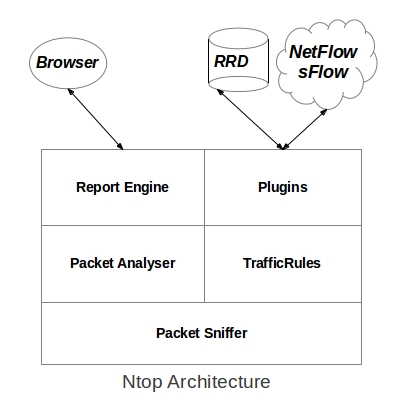
\includegraphics[scale=.5]{ntoparc.jpg}
          \caption{Architecture of \emph{ntop}.} 
        \end{figure}
	\subsection{Packet Analyzer}
	 \paragraph\
	 Packet Analyzer gets packets from Packet Sniffer and process those packets. Sniffed packets contained 
	 information about status of network and that information calculated by Packet Analyzer then stored in 
	 RRD for future references.
	\subsection{Traffic Rules}
	\paragraph\
	  \emph{ntop} allows user to specify what kind traffic a user is interested. Using \emph{libpcap} filter expression 
	  \emph{ntop} achieve this goal. Traffic Rules helps \emph{ntop} to reduce some burden on memory as well CPU, makes \emph{ntop}
	  more faster as it process less amount of packets.
	\subsection{Report Engine}
	\paragraph\
	  \emph{ntop} contains a web-server by which user from any geological location can monitor their network.
	  Report Engine provides a beautiful user interface with time series graph drawn using RRDTool. Using Report Engine
	  a user can change behavior of \emph{ntop} by changing its configuration parameters.
	\subsection{Plugins}
	 \paragraph\
	 \emph{ntop} has flexible design that allows user to add their own plugins. At startup \emph{ntop}
	 searches shared libraries (like .so, .dll files) to load  plugins. A plugin can access \emph{ntop}'s global 
	 data structure and can use API exported by \emph{ntop}.

      \section{Cassandra Database}
      \paragraph\
      Cassandra is a highly scalable and highly available database initially developed by Facebook using 
      two famous approach GFS\cite{gfs}  from Google and Dynamo\cite{dynamo} from Amazon. Cassandra currently highly
      used in ebay and Netflix. 
      Cassandra's big data features are 
      \begin{enumerate}
       \item Elastic scalability.
       \item High availability.
       \item Distributed database design with no single point of failure.
       \item Blistering linear performance.
       \item Multiple datacenter based data distribution.
      \end{enumerate}
      \paragraph{Why Cassandra:} In one of our testbed we are able to generate approx 1000 NetFlow packets per second with only two node
      having 1 Gbps NIC card. Bellow table provides amount of data generated by our testbed.\\
      \begin{tabular}{ccc}
      \\
      \hline
	  Packets generated& Time & Size of generated data \\
	  \hline
	  1000   & 1 second & 1.4MB\\
	  60 k   & 1 minute & 85 MB\\
	  3.6 m  & 1 hour    &  5 GB\\
      \end{tabular}\\
      It is clear that we can't use RDMS based databases for storing flow in data center network which can create explosive amount of
      data in short time. So for Flow monitoring a database should have following features:
      \begin{enumerate}
       \item Scalability : So that huge amount of data can be stored according to the demand.
       \item High write throughput : As flow records generate at rapid speed in data center network, it requires  to write
	     them fast.
       \item Reasonable read performance : For real-time processing.
       \item MapReduce support: For offline flow processing needs MapReduce for massive data crunching operation.
      \end{enumerate}
      
      Here is list of nosql databases that I have reviewed.
      
      \paragraph{Redis:} Redis is written in C. It has fast read-write performance but not scalable. Redis cluster
      going to lunch by end of 2013\cite{rrdcluster}, but for now it is out of consideration. 
      \paragraph{HBase:} HBase is written in Java . It is scalable, good read write performance but suitable for
      batch processing. It has single point of failure with Hadoop NameNode for which HBase may lose data  .  
      \paragraph{Cassandra:} Cassandra meet all the requirements that needed.
      
          \begin{figure}[htb]
	    \centering
	    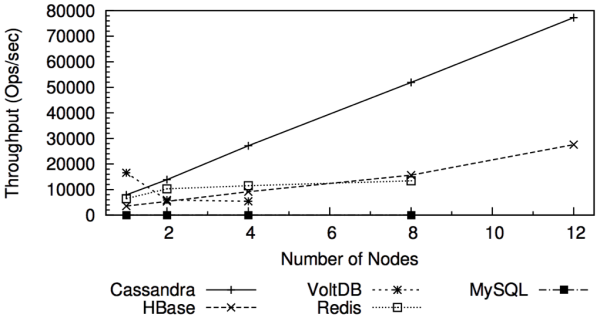
\includegraphics[scale=.5]{cassathpt.png}
	    \caption{Cassandra Performance\cite{cassathpt}.} 
	  \end{figure}
      
      \section{Cassandra C Client}
      \paragraph\
      Cassandra C client is a wrapper around Cassandra Python client that is Pycassa. I used C-Python API
      to write wrapper around Python's Pycassa API.   